\section{The Semantic Web Language Server}%
\label{sec:semantic_lsp}

The architectural design of the Semantic Web Language Server (SWLS) adheres to state-of-the-art implementation practices to ensure modularity, scalability, and maintainability~\cite{10.1145/3550355.3552452,10.1145/3563834.3567537,10.1145/3550355.3552452,Bour_2018}.
Unlike traditional architectures, SWLS leverages an entity component system (ECS), which offers greater separation of concerns compared to the widely recognized \textit{Layered Architecture}~\cite{10.1145/3550355.3552452}.

An ECS is a software design pattern that organizes a program into four key elements: Entities, Components, Systems, and Resources. 
In SWLS, \textit{entities} represent documents that are composed of various components. 
\textit{Components} store data associated with the entity, such as the document's contents, file location, or derived RDF triples. 
\textit{Systems} are functions designed to process specific components and are grouped into schedules to achieve distinct tasks. 
For example, the \textit{Parse} schedule includes systems responsible for tokenization, parsing, and triple extraction.
Semantic Web languages integrate seamlessly by introducing their systems into these predefined schedules to provide language-specific functionality.
\textit{Resources} are global components that are not linked to a specific entity.
For example, SWLS uses a resource to keep track of the hierarchy of discovered types, as types are not document specific.

As noted by Bour et al., ``No spec, no tests'' highlights the challenge of developing test suites for user-facing applications like language servers, where specifications can be open to interpretation~\cite{Bour_2018}. 
To address this, SWLS implements shared systems for common functionality, ensuring consistency and reducing redundancy across various Semantic Web languages.
By adopting this approach, SWLS delivers uniform features, while maintaining flexibility for language-specific extensions.

SWLS is implemented in Rust and leverages Bevy’s Entity Component System (ECS)\footnote{\url{https://bevyengine.org/}} to maintain a highly modular and efficient architecture.
Features are typically added in two steps:
  first, extracting the necessary data from RDF triples and attaching it to relevant entities; 
  second, using this data to implement language server functionalities such as diagnostics or autocompletion.

Bevy ECS facilitates this process by allowing the creation of isolated components and systems, enabling new features to be developed without impacting existing functionality.
This modularity ensures that only the minimal required data is extracted for each task, avoiding the complexity and overhead of constructing a complete digital twin of the document at hand.

For example, to implement autocompletion based on defined classes, two small systems are added:
  one to extract information about defined classes and their descriptions,
  and another to incorporate this information into autocompletion requests. 
Similarly, adding a feature to display type hierarchies would involve creating a system to extract data specific to the \texttt{rdfs:subClassOf} relation, without interfering with other systems.
This approach allows for scalable and focused development of language server features.

\subsection{Language Server Features}

This section lists all possible language features, according the protocol.
It also lists whether or not SWLS supports that feature and if that feature could be applied to semantic formats.

\begin{table}[ht]
  \centering
\makebox[\textwidth][c]{
\resizebox{1.5\textwidth}{!}{
\begin{tabular}{||l l l||} 
  \hline
  Feature & Supported? & Note \\ [0.5ex]
  \hline \hline
  Goto Declaration & No & Might be useful to jump to triples where the current term is in the subject position.\\ & & But it is unclear if this should be limited to only the curent document in the case of a named node, otherwise a lot of targets could be found. \\
  \hline
  Goto Definition & No & Allows jumping to OWL class or RDF property definitions \\
  \hline
  Goto Type Definition & No & Allows jumping to the OWL class definition of the type of the current term. \\
  \hline
  Goto implementation & No & This does not make any sense. \\
  \hline
  Find References & No & For a named node, this can resolve all uses of that named node, project wide. Or for a blank node in the current file. \\
  \hline
  Call hierarchy & No & This does not make any sense. \\
  \hline
  Type Hierarchy & Yes & Allows for following the \texttt{rdfs:subClassOf} property. \\
  \hline
  Document Highlight & No & Highlights the all terms that are the same term of at the current position. \\
  \hline
  Document Link & No & I guess that each named node is a link, but the actual usefulness of this is not clear. \\ & &  However the named nodes in prefix declarations might point to the actual ontology files, instead of the URI. \\
  \hline
  Hover & Yes & Adds additional information about the given position. \\
  \hline
  Code Lens & No & Might allow for inlining blank nodes or converting blank nodes to named nodes. \\
  \hline
  Folding Range & No & Triples or blanknodes with multiple predicate objects can be folded. \\
  \hline
  Select Range & No & A selection is the token at the given position. \\
  \hline
  Document Symbols & No & Each triple or blank node could be it's own symbol. \\
  \hline
  Semantic Tokens & Yes & Adds color information to all token in the document. \\
  \hline
  Inline Values & No & Adds no benefit.\\
  \hline
  Inlay Hints & Yes & Adds type information to terms.\\
  \hline
  Monikers & No & idk \\ 
  \hline
  Completion & Yes & Suggests completions based on current ontology and infered type. \\
  \hline
  Publish Diagnostics & Yes & Notifies the editor of syntax errors and shape violations. \\
  \hline
  Signature Help & No & Might suggest signatures according to some shape, suggestion required or optional properties for an object. \\
  \hline
  Code Action & Yes & Is used to fix problems lik undefined prefixes. Other code actions might be to inline a blank node. \\
  \hline
  Document Color & No & Adds no benefit. \\
  \hline
  Formatting & Yes & Allows for automatic formatting. \\
  \hline
  Rename & Yes & Allows for renaming terms. \\
  \hline
\end{tabular}
  }
  }
\end{table}




\subsection{Language Server schedules}

This section details the systems implemented within each schedule of SWLS.
Some systems are designed primarily to generate components, which are then utilized by other systems, potentially across different schedules.
This decoupled design ensures flexibility and modularity. 
If a system expects a component that is not present for a given entity, the system simply skips that entity.
For example, when parsing fails, a \texttt{Dirty} component is added to that entity.
Systems can then filter on all documents that do not have a \texttt{Dirty} component and execute their logic on them.

% this 
This greatly improves performance as when the user types the document is often broken.
This architecture supports asynchronous execution of systems, allowing for independent processing and reducing bottlenecks in the language server’s operation.
 %or this
This greatly improves performance as documents are often broken when they are edited.
The ECS architecture supports asynchronous execution of systems, allowing for independent processing and reducing bottlenecks in the language server’s operation.

\subsubsection{Parse}

\begin{figure}[tb]
 \centering
 \makebox[\textwidth]{%
    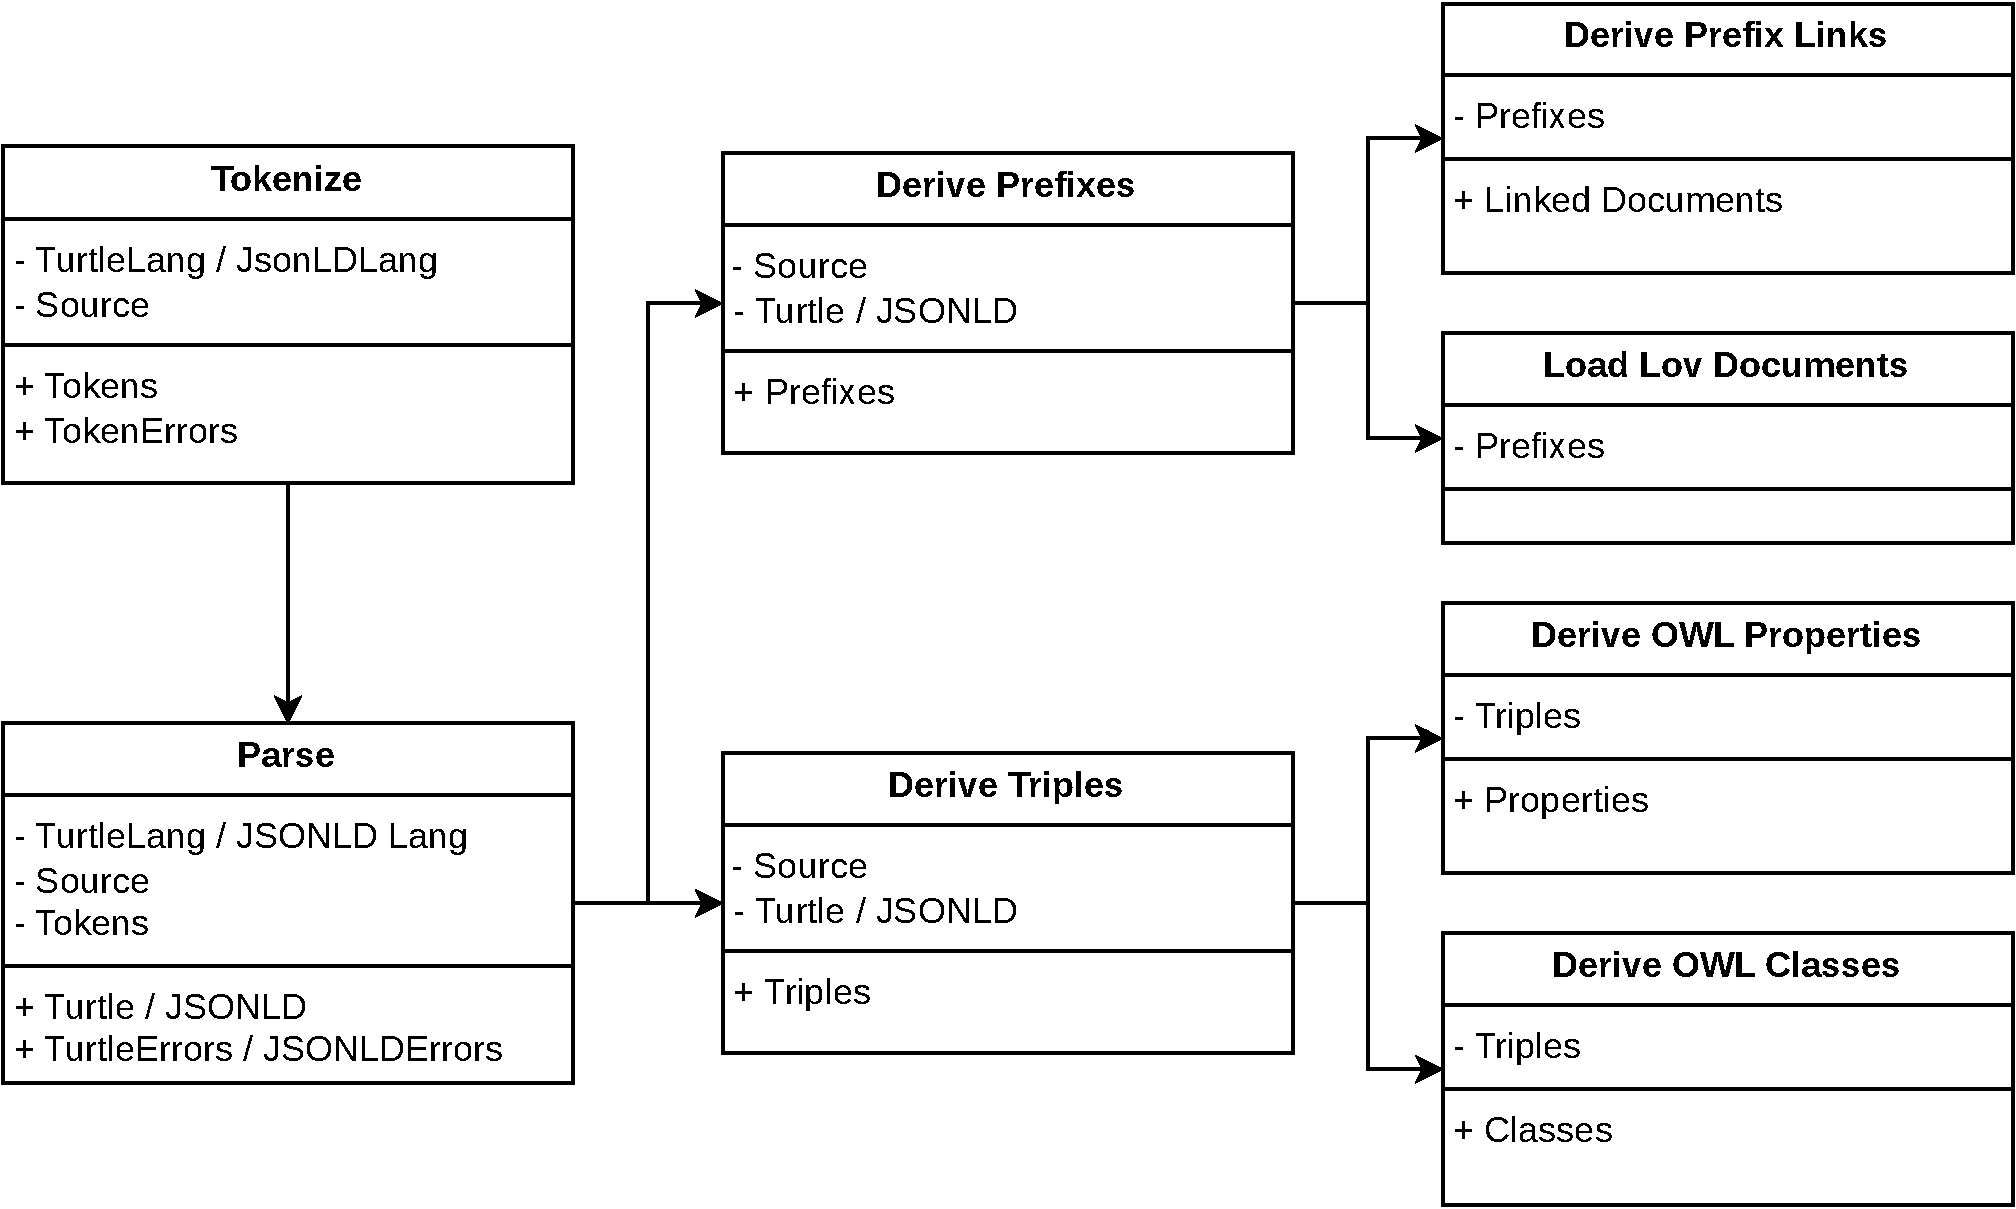
\includegraphics[width=1.2\textwidth]{./images/ParseSchedule.pdf}
 }
  \caption{Visual representation of the Parse schedule including tokenization, parsing, deriving prefixes, deriving triples, linking documents, fetching LOV documents, deriving properties and deriving classes. }\label{fig:Parse}
\end{figure}

The \textit{Parse} schedule %is one of the most important schedules of SWLS. It % → Aren’t they all?
is activated whenever the user edits a document, notifying the language server of the textual changes.

We chose to let all semantic languages use the same \texttt{token} type. 
This allows for implementing token-based systems only once.
Note, that this does not mean SPARQL specific tokens (i.e. \texttt{?variable} or SPARQL keywords) are introduced into the Turtle language:  each language does their own tokenization, merging all tokens into one \texttt{token} type.
In Figure~\ref{fig:Parse}, \textit{tokenize} is the first system in the parsing schedule, this system is implemented for all supported languages. \textit{Tokenize} also reports on tokenization errors.

The next system is \textit{parsing}, also implemented for each semantic language, transforming the tokens into actual objects and reporting on syntactic errors. 
When the objects are parsed, systems are issued to derive prefixes and triples. 
Prefixes contain information about how to expand and shorten IRIs for the current document.
Deriving triples does not only derive actual RDF triples, but in the case of SPARQL, also triple patterns with variables, which can be thought of as \textit{triples}.

<<<<<<< HEAD
After deriving prefixes, other systems will create a \texttt{LinkedDocuments} component, listing all documents that are linked in some way to this document.
Prefixes are one way, but the object value of the following triple also allows linking the document on the otherLocation with the current document.
\begin{verbatim}
  <> owl:imports <otherLocation>.
\end{verbatim} 
=======
When the triples are derived, the next systems will derive properties and classes.
These properties and classes are later used to suggest autocompletions and derive type hierarchies.
>>>>>>> f163990 (last changes)

SWLS introduces the concept of linked documents, documents that are related to the current document, which should be used for features like autocompletion.
Prefix statements are one way to link documents, but the object value of the triple \texttt{<> owl:imports <otherLocation>.}, also allows linking that other document with the current document.
To acquire useful properties and classes, SWLS looks for ontology files, however we noticed that dereferencing the location of a prefix statement and expecting an ontology file is actually quite rare, 
so we introduced the LOV~\cite{LOV2017} service into SWLS.
Given a prefered prefix, SWLS will try to retrieve an ontology file from LOV and insert it into the language server.
This triggers the parsing schedule again for that document, deriving the actual properties and classes.

\todo{help}
SWLS uses LOV\cite{LOV2017} to access ontologies definitions that are imported as a prefix of a document.
These ontology documents are loaded into the language server as normal editor documents
This means that properties and classes are derived from ontology documents or local documents.
Prefixes are also used to load the correct LOV~\cite{LOV2017} defined ontologies, setting up documents containing property and class definitions.~\info{this comes out of the blue. We need to properly describe that LOV is used internally used to support a richer set of ontologies and specially those that are not dereferenceable.}

The language server protocol allows the server to specify wether it requires only the (minimal) changes or the entire document every time.
Earlier versions of the SWLS required the entire document every time, given that documents are usually small and reprasing the entire document could be done with an acceptable performance.
However, we noticed that this hampered the implementation, in Turtle specifically there are patterns that cannot be parsed correctly and brings incorrect and frustrating feedback to the user, and partial parsing helps in this regard.
An example is shown in Figure~\ref{lst:GroupedListing}.
  (i) The user at figure \ref{code1} types the named node \texttt{<b>}. The language server should determine that triple \texttt{<c> <d> <e>} has nothing to do with named node \texttt{<b>} and should suggest objects that fulfill the range of predicate \texttt{<b>}. 
  (ii) The user at figure \ref{code2} types the named node \texttt{<c>}. The language server should identify that the are two triples \texttt{<a> <b> <c>} and \texttt{<a> <d> <e>}. Although token-wise documents in figures~\ref{code1} and \ref{code2} are the same, in this case the suggestion should result in a semicolon.
  (iii) The user at figure \ref{code3} just wrote subject \texttt{<a>}, invoking the subject completion defined in the next section.
     The language server might incorrectly suggest to add a comma after \texttt{<c>} to build a syntactically correct document. 
     This however would be a mistake as triple \texttt{<b> <c> <d>} has \texttt{<b>} as subject, not \texttt{<c>}.
  (iv) The user at figure \ref{code4} is typing the predicate \texttt{<b>} for the subject \texttt{<a>}, the language server might incorrectly parse the document as seen at figure~\ref{code3}, where \texttt{<b>} is subject thus not suggesting the property completion as explained in the next section.

  Adding partial parsing can deal with these issues as the language server understand which tokens are added or deleted and leaving the original interpretation of the surrounding tokens untouched.

\begin{figure}[tb]
    \centering
    % code1
    \begin{subfigure}{0.21\textwidth}
      \lstinputlisting{./code/option1.ttl}
      \caption{User types predicate \texttt{<b>}}
      \label{code1}
    \end{subfigure}
    \hfill
    % code 2
    \begin{subfigure}{0.21\textwidth}
      \lstinputlisting{./code/option2.ttl}
      \caption{User types object \texttt{<c>}}
      \label{code2}
    \end{subfigure}
    \hfill
    % code 3
    \begin{subfigure}{0.21\textwidth}
      \lstinputlisting{./code/option3.ttl}
      \caption{User types subject \texttt{<a>}}
      \label{code3}
    \end{subfigure}
    \hfill
    % code 4
    \begin{subfigure}{0.21\textwidth}
      \lstinputlisting{./code/option4.ttl}
      \caption{User types predicate \texttt{<b>}}
      \label{code4}
    \end{subfigure}
    \caption{Different code samples showing that it is the indentation/intent of the user that dictates how tokens should be parsed. (a) and (b) show five terms that result in different triples. (c) and (d) show four terms, triples with subject \texttt{<a>} and \texttt{<b>} and both triples with subject \texttt{<a>} resulting in different semantics.    }\label{lst:GroupedListing}
\end{figure}
% The language server protocol allows the server to specify wether it requires only the (minimal) changes or the entire document every time.
% Earlier versions of the SWLS required the entire document every time, given that documents are usually small and reprasing the entire document could be done with an acceptable performance.
% However, we noticed that this hampered the implementation, in Turtle specifically there are patterns that cannot be parsed correctly and brings incorrect and frustrating feedback to the user, and partial parsing helps in this regard.
% An example is shown in Figure~\ref{lst:GroupedListing}.
%   (i) The user at figure \ref{code1} types the named node \texttt{<b>}. The language server should determine that triple \texttt{<c> <d> <e>} has nothing to do with named node \texttt{<b>} and should suggest objects that fulfill the range of predicate \texttt{<b>}. 
%   (ii) The user at figure \ref{code2} types the named node \texttt{<c>}. The language server should identify that the are two triples \texttt{<a> <b> <c>} and \texttt{<a> <d> <e>}. Although token-wise documents in figures~\ref{code1} and \ref{code2} are the same, in this case the suggestion should result in a semicolon.
%   (iii) The user at figure \ref{code3} just wrote subject \texttt{<a>}, invoking the subject completion defined in the next section.
%      The language server might incorrectly suggest to add a comma after \texttt{<c>} to build a syntactically correct document. 
%      This however would be a mistake as triple \texttt{<b> <c> <d>} has \texttt{<b>} as subject, not \texttt{<c>}.
%   (iv) The user at figure \ref{code4} is typing the predicate \texttt{<b>} for the subject \texttt{<a>}, the language server might incorrectly parse the document as seen at figure~\ref{code3}, where \texttt{<b>} is subject thus not suggesting the property completion as explained in the next section.
%
%   Adding partial parsing can deal with these issues as the language server understand which tokens are added or deleted and leaving the original interpretation of the surrounding tokens untouched.
%
% \begin{figure}[tb]
%     \centering
%     % code1
%     \begin{subfigure}{0.21\textwidth}
%       \lstinputlisting{./code/option1.ttl}
%       \caption{User types predicate \texttt{<b>}}
%       \label{code1}
%     \end{subfigure}
%     \hfill
%     % code 2
%     \begin{subfigure}{0.21\textwidth}
%       \lstinputlisting{./code/option2.ttl}
%       \caption{User types object \texttt{<c>}}
%       \label{code2}
%     \end{subfigure}
%     \hfill
%     % code 3
%     \begin{subfigure}{0.21\textwidth}
%       \lstinputlisting{./code/option3.ttl}
%       \caption{User types subject \texttt{<a>}}
%       \label{code3}
%     \end{subfigure}
%     \hfill
%     % code 4
%     \begin{subfigure}{0.21\textwidth}
%       \lstinputlisting{./code/option4.ttl}
%       \caption{User types predicate \texttt{<b>}}
%       \label{code4}
%     \end{subfigure}
%     \caption{Different code samples showing that it is the indentation/intent of the user that dictates how tokens should be parsed. (a) and (b) show five terms that result in different triples. (c) and (d) show four terms, triples with subject \texttt{<a>} and \texttt{<b>} and both triples with subject \texttt{<a>} resulting in different semantics.    }\label{lst:GroupedListing}
% \end{figure}



\subsubsection{Completion}

\textit{Completion} is one of the most prominent feature actively interacting with the user.
In LSP, the server receives a completion event that contains the current cursor location of the user.
The server should then answer with a list of completions, including the textual operations, a title and potentially some documentation.
It is the responsibility of the editor to sort and filter the completions and show the user the most relevant information.
How editors do this is not specified, which makes it difficult to create comprehensive and cross-IDE testing suites.

\begin{figure}[!ht]
 \centering
 \makebox[\textwidth]{%
    \includegraphics[width=1.2\textwidth]{./images/Completion.pdf}
 }
  \caption{Visual representation of the Completion schedule including GetCurrentToken, GetCurrentTriple, Subject Completion, Defined Prefix Completion, Prefix.cc Prefix Completion, Complete Classes and Complete Properties.}\label{fig:Completion}
\end{figure}

Figure~\ref{fig:Completion} shows a schematic overview of the different systems involved in the completion schedule and their interactions.
First the server will create a \texttt{CompletionRequest} object, at first containing no completions.
Systems will proceed to add their relevant completions to the request which is then returned to the user.

The location the user is at the moment of the request, is not enough information to derive comprehensive completions. 
The first systems will extract more information, with \texttt{GetCurrentToken} and \texttt{GetCurrentTriple}, which is then used by the systems that create the actual completions.

\texttt{GetCurrentToken} expands the current location to the current token, then \texttt{GetCurrentTriple} tries to find the triple that this token belogns to, and also to identify whether the user is typing a subject, predicate or object.
If \texttt{GetCurrentToken} fails, the entity lacks a TokenComponent and results in \texttt{GetCurrentTriple} not being issued. 
This happens when the user issues a completion request, but the cursor is standing in whitespace.
\texttt{GetCurrentTriple} might fail if the user is editing parts of the document that is not an actual triple, like a prefix statement.

The language server has enough information with only the current token to complete based on defined subjects, which can be seen as entities defined in the document, with the \texttt{SubjectCompletion} system.
The server also completes on already defined prefixes (with \texttt{Comlete Defined Prefix}), this system is language agnostic as the Prefixes component is already extracted during the Parse schedule.
To suggest importing new prefixes, SWLS uses Prefix.cc\footnote{\url{https://prefix.cc}}, an online service that maps prefered prefixes to IRIs.
This system is implemented for each language, as the actual edits that should be applied to the document is langauge specific.

SWLS will also suggest properties, if \texttt{GetCurrentTriple} identified that the user is writing a predicate.
To give the best suggestions, SWLS tries to determine the type of the current subject, currently SWLS only looks for the \texttt{rdf:type} predicate. 
If a type is found, SWLS orders properties in such a way that properties with the correct domain are shown first,
and visually distinguishes them from other properties.
When the user is typing an object and the predicate of the current triple is \texttt{rdf:type}, SWLS suggests defined classes.


\subsubsection{Diagnostics}

The \textit{Diagnostics} component of SWLS comprises several focused systems that analyze parsed data to identify issues and provide feedback to users.
Diagnostics differ fundamentally from other language server functionalities because they are push-based: the server actively notifies the editor of errors and warnings.
This allows for timely feedback, ensuring that users can quickly identify and address problems in their documents.

Diagnostics are triggered with two different schedules: \textit{on-edit} and \textit{on-save}.

\begin{enumerate}
  \item \textit{On edit} diagnostics provide fast, real-time feedback to users, enabling them to fix errors as they type. 
    This ensures a fluid editing experience and minimizes interruptions.
  \item \textit{On save} diagnostics occur less frequently and are therefore better suited to more computationally intensive checks,
   such as validation against SHACL shapes.
\end{enumerate}

To demonstrate the capabilities of the diagnostics system, we highlight three key systems:

\begin{enumerate}
  \item \textit{Syntax Diagnostics:}
    During the tokenization and parsing phases, errors such as syntax mismatches or malformed input are detected and recorded, along with their locations.
    These errors are immediately passed to the diagnostics publisher resource, making this part of the on-edit schedule, as the necessary data is already generated during parsing.
  \item \textit{SHACL Validation:} 
    With the on save schedule, the server uses the Rudof library\footnote{\url{https://github.com/rudof-project/rudof}} to validate the current RDF document against SHACL and SHEX shapes~\cite{labra2022rudof}.
    Shapes are dynamically extracted from the document itself (if present), as well as other linked documents.
    This system ensures that the semantic data conforms to expected structural constraints, enabling robust validation for ontologies and RDF documents.
  \item \textit{Basic Validation:}
    This system identifies common issues, such as undefined prefixes or unused declarations.
    By flagging such problems, users can better maintain consistency and avoid errors that might lead to interoperability issues.
\end{enumerate}

Together, these systems provide comprehensive diagnostic support, catering to both immediate feedback needs and more in-depth validation processes.
This modular approach ensures that diagnostics remain lightweight yet powerful, accommodating the diverse requirements of Semantic Web practitioners.

\subsubsection{Others}

Beyond core functionalities, SWLS offers additional schedules that enhance the user experience and round out its capabilities.
These schedules are smaller in scope, generally focusing on presentation or user interaction rather than deriving new information.

The most notable are as follows:
\begin{enumerate}
  \item \textit{Formatting:}
    A consistent document structure improves readability and reduces the cognitive load required to parse data visually.
    As a formatter, the language server ensures uniformity across documents, promoting best practices and easing collaboration.
    Currently, the SWLS includes an opinionated formatter for Turtle, which automatically applies a standardized layout to documents.

  \item \textit{Hover:}
    Hover functionality provides contextual insights about symbols in the document, offering users additional information without disrupting their workflow,
    allowing for users to explore semantic relationships and documentation seamlessly.
    The SWLS’s hover implementation includes three key features:
    \begin{itemize}
      \item Type Information: For a node with an inferred type, the hover popup displays the type alongside its hierarchy, including subclasses and superclasses.
      \item Class Details: Hovering over a class reveals its \texttt{rdfs:description}.
      \item Property Insights: Hovering over a property shows its \texttt{rdfs:description}, as well as its range and domain.
    \end{itemize}

  \item \textit{Highlighting:}
    Highlighting improves document readability by visually distinguishing between elements.
    The SWLS implements both syntax highlighting and semantic highlighting through a two-step process:
        (i) An initial system maps all tokens to their basic semantic types.
        (ii) Subsequent systems refine the types based on additional information.
    For example, in JSON-LD, all keys are initially highlighted as strings.
    However, keys starting with the \texttt{@} symbol are reclassified as keywords, enhancing clarity and usability for JSON-LD documents.
\end{enumerate}

These schedules, while smaller in scale, significantly enhance the language server’s utility by making semantic documents more intuitive and easier to work with.
They represent the \textit{polish} that transforms SWLS into a complete tool for Semantic Web practitioners.
